\documentclass[../Master.tex]{subfiles}
\begin{document}
\chapter{Experimental section}\label{cha:experimental-section}
\section{Dimethyl 4,4'-malonyldibenzoate}
\subsection{Synthesis}

\begin{center}
	\begin{tabular}[b]{lccccccc}
		\toprule
		Reagent                 & CAS       & MW / \(g \ mol^{-1}\) & m / g & n / mmol & SR   \\
		\midrule
		methyl 4-acetylbenzoate & 3609-53-8 & 178.19                & 4.400 & 24.69    & 1.20 \\
		dimethyl terephthalate  & 120-61-6  & 194.19                & 4.000 & 20.60    & 1.00 \\
		NaH, mineral dispersion & 7646-69-7 & 23.998                & 1.132 & 47.17    & 2.30 \\
		\bottomrule
	\end{tabular}
\end{center}

The reaction is carried out under N$_{2}$ atmosphere, the reactant are carefully dried beforehand.\\
In a flask, 1.132 g of NaH dispersion in mineral oil are washed with anhydrous THF (15 mL x 2).\\
4.0 g of methyl 4-acetyl benzoate and 4.4 g of dimethyl terephthalate are dissolved in 45 mL of anhydrous THF, and then NaH suspension in THF is added.\\
The mixture is heated to reflux overnight. \\
Evaporation of the solvent under vacuum gives a dark brown compound. The solid is taken up in water and acidified with HCl 20\% in an ice bath. Taking care to leave it to react for a few hours and checking the pH to make sure it is acid. More water is added if mixing is particularly difficult.\\
The raw product is recovered as a yellow solid by filtration with a Buchner funnel.
To eliminate the impurities of the remaining reagents the solid is washed with chloroform and with diethyl ether. The solid is lastly collected on a Buchner funnel and dried. Yield: 92\%, 8.67 g of product.
\subsection{Characterization}
\subsubsection{NMR}
\subsubsection{IR}
\section{4,4'-malonyldibenzoic acid}
\subsection{Synthesis}

\begin{center}
	\begin{tabular}[b]{lccccccc}
		\toprule
		Reagent                         & CAS       & MW / \(g \ mol^{-1}\) & m / g & n / mmol & SR \\
		\midrule
		Dimethyl 4,4'-malonyldibenzoate & -         & 340.31                & 1.000 & 2.940    & 1  \\
		LiOH                            & 1310-65-2 & 23.95                 & 1.411 & 58.80    & 20 \\
		\bottomrule
	\end{tabular}
\end{center}

In a small beaker, 1.411 g of freshly ground LiOH is dissolved in 10 mL of water. In an flask, 1.000 g of 4,4'-malonyldibenzoate is suspended in 10 mL of THF, then the LiOH solution is slowly added. The mixture is allowed to react 7 hours at room temperature under vigorous stirring. It is then proceeded by extracting with \(CHCl_{3}\) (3x25 mL). The aqueous phase is collected and acidified with 10 \% HCl to acidic pH, observing the formation of straw-yellow precipitate. The solid is recovered by filtration over buchner and allowed to air dry.

\subsection{Characterization}
\subsubsection{NMR}
\subsubsection{IR}
\section{Methyl 4,4'-(1H-pyrazole-3,5-diyl)dibenzoate}
\subsection{Synthesis}
\subsubsection{EtOH}
A typical synthesis is described here:
500 mg of dimethyl 4,4'-malonyldibenzoate is suspended in 20 mL of EtOH in a 50 mL flask. The mixture is left in ultrasonic bath for 30'. 350 \(\mu L\) of hydrazine monohydrate are slowly added to the mixture that is then heated to reflux overnight.\\
The compound is collected as a pale yellow solid on a teflon funnel. Yield: 25\%.
\subsubsection{DMF}
500 mg of dimethyl 4,4'-malonyldibenzoate is suspended in 15 mL of DMF in a 50 mL flask. The mixture is left in ultrasonic bath for 30'. 350 \(\mu L\) of hydrazine monohydrate are slowly added to the mixture that is then heated to 150°C overnight.\\
Evaporation of the solvent under vacuum gives a white ivory solid. The compound is then washed adding 25 mL of ethanol and heat to reflux for 2 hours. Pure solid is collected on a Buchner funnel. Yield: 48\%.
\subsubsection{DMSO}
500 mg of dimethyl 4,4'-malonyldibenzoate is solubilized in 20 mL of DMSO in a 50 mL flask. The mixture is left in ultrasonic bath for 30'. 350 \(\mu L\) of hydrazine monohydrate are slowly added to the mixture that is then heated to 150°C overnight.\\
\pagebreak
\subsection{Characterization}
\subsubsection{NMR}
\subsubsection{IR}

\section{4,4'-(1H-pyrazole-3,5-diyl)dibenzoic acid}
\subsection{Synthesis}
\subsubsection{LiOH}
\begin{center}
	\begin{tabular}[b]{lccccccc}
		\toprule
		Reagent                                   & CAS       & MW / \(g \ mol^{-1}\) & m / g  & n / mmol & SR \\
		\midrule
		4,4'-(1H-pyrazole-3,5-diyl)dibenzoic acid & -         & 336.47                & 0.3023 & 0.8988   & 1  \\
		LiOH                                      & 1310-65-2 & 23.95                 & 0.4505 & 17.796   & 20 \\
		\bottomrule
	\end{tabular}
\end{center}

In a small beaker, 0.4505 g of freshly ground LiOH is dissolved in 6 mL of water. In an flask, 0.3023 g of methyl 4,4'-(1H-pyrazole-3,5-diyl)dibenzoate is suspended in 6 mL of THF, then the LiOH solution is slowly added. The mixture is allowed to react overnight at room temperature under vigorous stirring. It is then proceeded by extracting with \(CHCl_{3}\) (3x25 mL). The aqueous phase is collected and acidified with 10 \% HCl to acidic pH, observing the formation of white precipitate. The solid is recovered by filtration over buchner and allowed to air dry.

\subsection{Characterization}
\subsubsection{NMR}
\subsubsection{IR}
\section{4,4'-malonyldibenzonitrile}
\subsection{Synthesis}
\begin{center}
	\begin{tabular}[b]{cccccccc}
		\toprule
		Reagent                & CAS       & MW / \(g \ mol^{-1}\) & m / g  & n / mmol & SR   \\
		\midrule
		methyl 4-cyanobenzoate & 1129-35-7 & 161.16                & 4.0370 & 25.05    & 0.93 \\
		4-acetylbenzonitrile   & 1443-80-7 & 145.16                & 3.3862 & 23.32    & 1.00 \\
		NaH                    & 7646-69-7 & 23.998                & 2.7780 & 115.75   & 4.96 \\
		\bottomrule
	\end{tabular}
\end{center}
The reaction is carried out under N$_{2}$ atmosphere, the reactant are carefully dried beforehand.\\
In a flask, 2.778 g of NaH dispersion in mineral oil are washed with anhydrous THF (15 mL x 2).\\
4.0370 g of methyl 4-cyanobenzoate and 3.3862 g of 4-acetylbenzonitrile are dissolved in 45 mL of anhydrous THF, and then NaH suspension in THF is added under ice bath while vigouros mixing. \\
The mixture is allowed to reach room temperature and then is heated to reflux overnight. \\
Evaporation of the solvent under vacuum gives a dark green compound. The solid is taken up in water and acidified with HCl 20\% in an ice bath. Taking care to leave it to react for a few hours and checking the pH to make sure it is acid. More water is added if mixing is particularly difficult.\\
The raw product is recovered as a yellow solid by filtration with a Buchner funnel.
To eliminate the impurities of the remaining reagents the solid is washed with ethanol. The solid is lastly collected on a Buchner funnel and dried. Yield: 74\%, 4.76 g of product.
\pagebreak

\subsection{Characterization}
\subsubsection{NMR}
\subsubsection{IR}
\begin{figure}[h!]
	\centering
	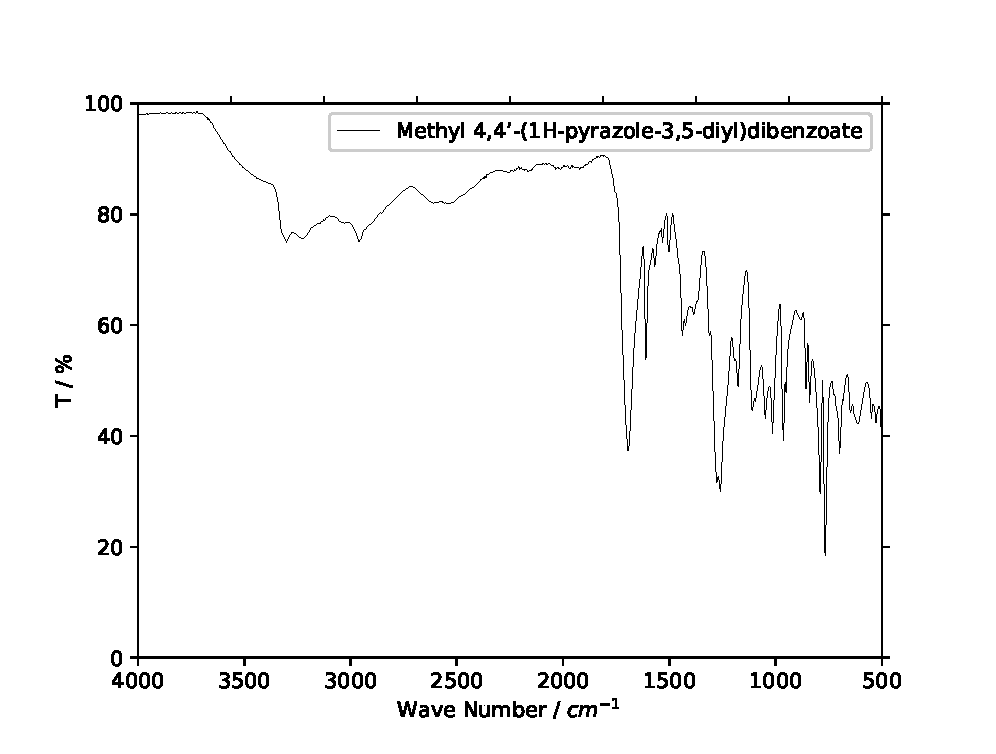
\includegraphics[width=20cm,height=10cm,keepaspectratio]{Spectra/pyr-est.eps}
\end{figure}

\section{Methyl 4‐[(1E)‐3‐[4‐(methoxycarbonyl)phenyl]‐3‐oxoprop‐1‐en‐1‐yl]benzoate}
\subsection{Synthesis}
\begin{center}
	\begin{tabular}[b]{cccccccc}
		\toprule
		Reagent                 & CAS       & MW / \(g \ mol^{-1}\) & m / g & n / mmol & SR  \\
		\midrule
		methyl 4‐formylbenzoate & 1571-08-0 & 178.18                & 0.500 & 2.8      & 1   \\
		methyl 4‐acetylbenzoate & 3609-53-8 & 164.16                & 0.550 & 3.5      & 1.2 \\
		NaOH                    & 1310-73-2 & 39.998                & 0.230 & 5.6      & 2   \\
		\bottomrule
	\end{tabular}
\end{center}

In a small beaker, 230 mg of freshly ground NaOH is dissolved in 10 mL of methanol. \\
In a flask, 500 mg methyl 4-formylbenzoate and 550 mg methyl 4-acetylbenzoate are dissolved in 5 mL MeOH. The mixture is placed under vigorous stirring in an ice bath. The freshly prepared sodium hydroxide solution is slowly added. The reaction is left to react overnight. \\
The yellowish solid is collected on Buchner funnel and allowed to air dry. Yield 94\%, 0.85 g of product.

\subsection{Characterization}
\subsubsection{NMR}
\end{document}
%%% Local Variables:
%%% mode: latex
%%% TeX-master: "../Master"
%%% End:

